\documentclass[10pt,xcolor=table]{beamer}

\usepackage[utf8]{inputenc} 
\usepackage[T1]{fontenc}
\usepackage{lmodern}
\usepackage{graphicx}
\usepackage[english]{babel}
\usepackage{array}
\usepackage{multirow}
\usepackage{stmaryrd}
\usepackage{tikz}
\usepackage{pgfplots}
\usepackage{manfnt}
\usepackage{enumitem}
\usepackage{hyperref}
\usepackage{transparent}
\usepackage{physics}
\usepackage{bm}
\usepackage[controls]{animate}
\usepackage[backend=biber,style=alphabetic,sorting=none]{biblatex}
\usepackage{csquotes}
\usepackage{ragged2e}
\usepackage{appendix}
\addbibresource{references.bib}

\usepackage{xcolor}
\definecolor{PLBfonce}{rgb}{0.06,0.42,0.60}
\definecolor{PLBmoyen}{RGB}{176, 216, 232}
\definecolor{PLBpale}{rgb}{0.94,0.965,0.965}

\setbeamercolor{frametitle}{bg=PLB}
\setbeamercolor{sidebar}{bg=PLB}
\setbeamercolor{logo}{bg=PLB!70!black}
\setbeamercolor{structure}{fg=PLB, bg=PLB!40}
\setbeamertemplate{footline}[frame number]
\setbeamertemplate{navigation symbols}{}
\setbeamercolor*{sidebar}{fg=red,bg=PLB!40!white}

\definecolor{PLB}{rgb}{0.06,0.42,0.60}

\theoremstyle{definition}

\newcommand{\timecolor}{red!80!black}
\newcommand{\spacecolor}{PLB!95!white}
\newcommand{\boundarycolor}{green!50!black}
\newcommand{\interiorcolor}{magenta!70!black}
\newcommand{\initialcolor}{orange!80!black}
\renewcommand*{\bibfont}{\scriptsize}
\newcommand{\backupbegin}{
	\newcounter{finalframe}
	\setcounter{finalframe}{\value{framenumber}}
}
\newcommand{\backupend}{
	\setcounter{framenumber}{\value{finalframe}}
}

\usetheme{PaloAlto}
\usefonttheme[onlymath]{serif}

\title[Evolution of OQS under continuous measurement of their environment]{Evolution of open quantum systems under continuous measurement of their environment}
\author[]{J.~Stevenot \and supervised by B.~Bellomo\inst{1}}
\date{June 2026}
\institute{\inst{1}Equipe $\Phi$Th, Institut UTINAM - CNRS 6213, OSU THETA}
\logo{
\includegraphics[height=9mm]{Images/logocomp.png}}

\pgfplotsset{compat=1.18}
\begin{document}

\begin{frame}
    \titlepage
    
    % Positionnement absolu des logos en bas de la page
    \begin{tikzpicture}[remember picture, overlay]
        \node[anchor=south west, xshift=1.7cm, yshift=0pt] at (current page.south west) {
            
\includegraphics[height=1.7cm]{Images/logoUTI.jpeg}
        };
        \node[anchor=south east, xshift=-0.1cm, yshift=0.4cm] at (current page.south east) {
            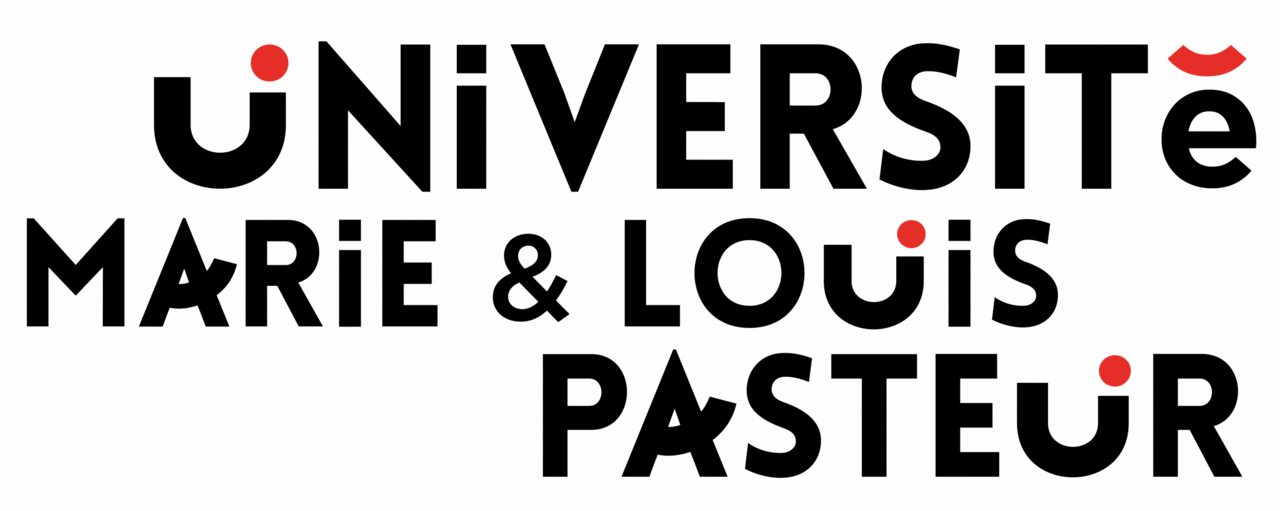
\includegraphics[height=1cm]{Images/logo.png}
        };
    \end{tikzpicture}
\end{frame}
\begin{frame}
	\frametitle{Table of contents}
	\tableofcontents
\end{frame}

\section{The context}
\subsection{Problem statement}
\begin{frame}
	\frametitle{Wave function collapse}
	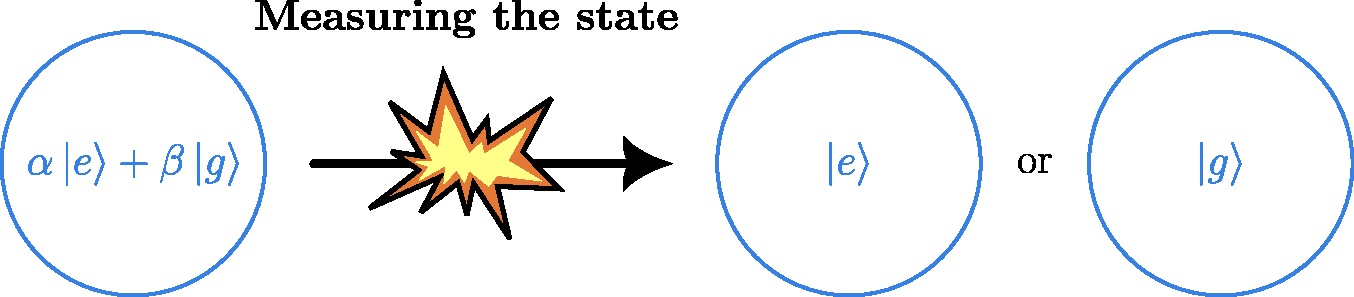
\includegraphics[width=\textwidth]{Images/Collapse.pdf}
	\vfill
	\begin{alertblock}{The main effect of measurements}
		Measuring a quantum system impacts its state.\\ In particular, it collapses onto one of the possible eigenstates.
	\end{alertblock}
\end{frame}

\subsection{The OQS theory}
\begin{frame}{The input-output formalism}
	\centering
	\only<1>{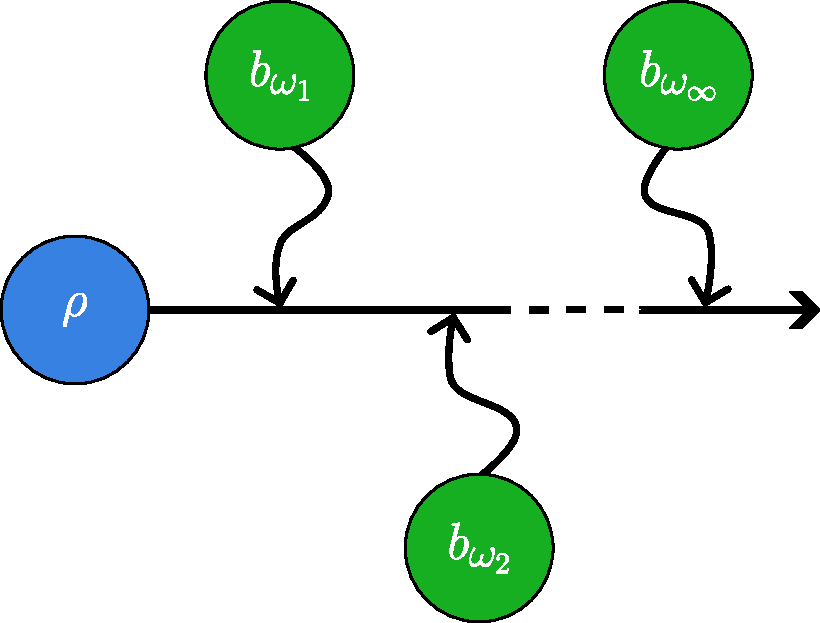
\includegraphics[width=\textwidth]{Images/Collisional.pdf}}
	\only<2>{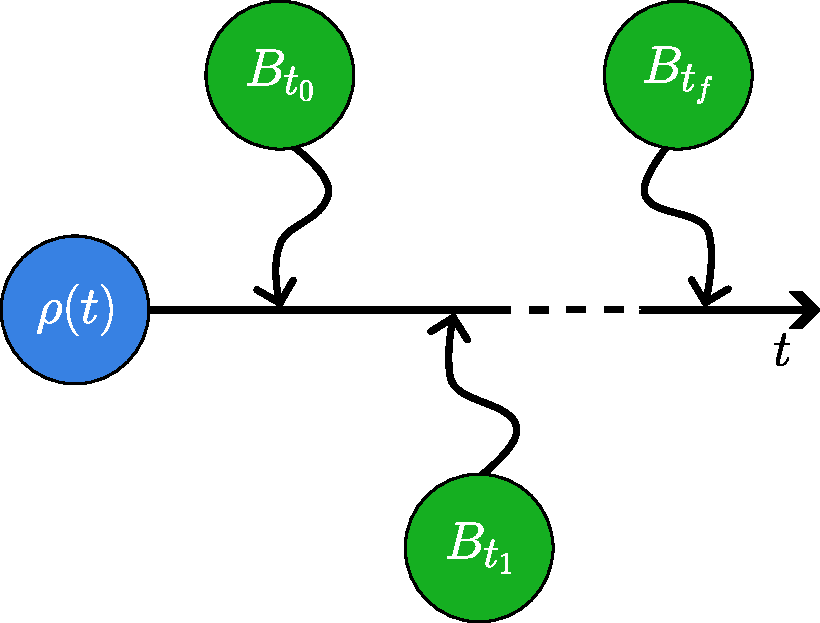
\includegraphics[width=0.5\textwidth]{Images/InputOutput.pdf}
	\begin{block}{The temporal input mode $b_t$~\cite{Carmichael}}
		\begin{gather*}
			b_t=\frac{1}{\sqrt{2\pi}}\int_\mathcal{W} b_\omega e^{-i(\omega-\omega_0)(t-t_0)}\mathrm{d}\omega,\\[0.4cm]
			\qty[b_t, b_{t'}^\dagger]=\delta(t-t')\quad\Longrightarrow\quad\qty[B_t,B_{t}^\dagger]=\mathbb{I}.
		\end{gather*}
	\end{block}
	}
\end{frame}
\begin{frame}
	\frametitle{The unconditional evolution}
	Under the approximations~\cite{Albarelli, WM}:
	\begin{itemize}[label=$\bullet$]
		\item<1-> constant coupling $\forall\omega\in\mathcal{W},\quad k(\omega)=k\in\mathbb{R}$ (named the first Markovian assumption),
		\item<2-> weak coupling condition $k\ll\omega_0$,
		\item<3-> operators acquire a time-dependant phase in the interaction picture $\tilde{c}(t)=c e^{-i\omega_0 (t-t_0)}$,
		\item<4-> the Born-Markov approximation $\forall t\in\mathbb{R},\quad \tilde{\bm{\varrho}}(t)=\tilde{\rho}(t)\otimes\ketbra{0}_t$.
	\end{itemize}
\end{frame}
\begin{frame}
	\frametitle{The unconditional evolution}
	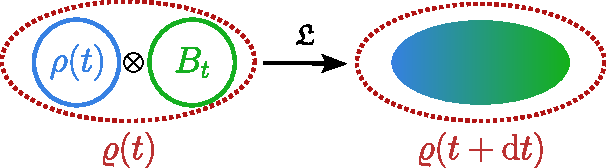
\includegraphics[width=\textwidth]{Images/OQS.pdf}
	\vfill
	\begin{block}{The Lindblad master equation~\cite{Breuer}}
		\begin{equation*}
			\frac{\mathrm{d}\rho}{\mathrm{d}t}(t) = -\frac{i}{\hbar}\qty[H_S, \rho(t)]+k\mathfrak{D}[c]\rho(t).
		\end{equation*}
	\end{block}
	We define the dissipator as $\mathfrak{D}[c]\rho=c\rho c^\dagger -\frac{1}{2}\qty(c^\dagger c \rho+\rho c^\dagger c)$.
\end{frame}

\section{Continuous measurement of the environment}
\subsection{Weak measurements}
\begin{frame}
	\frametitle{Avoiding the brutal collapse of the system's state}
	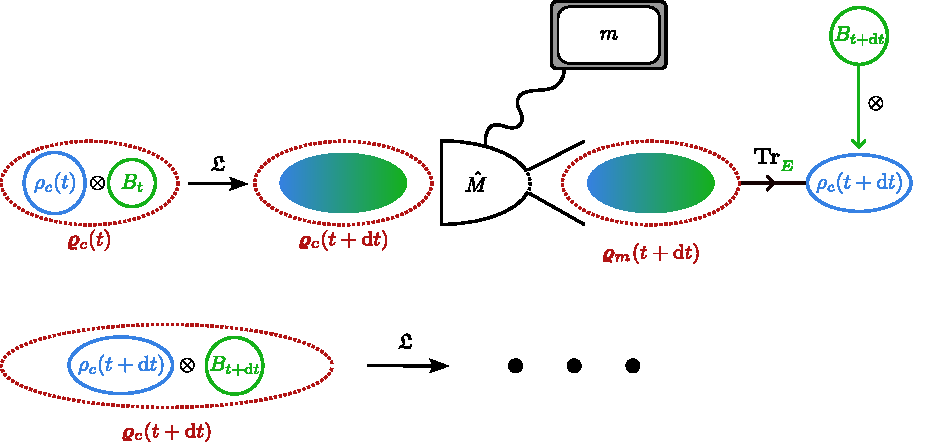
\includegraphics[width=\textwidth]{Images/Scheme.pdf}
	\vfill\centering\pause
	\begin{block}{The evolution of the total state $\bm{\varrho}$}
		\begin{equation*}
			\bm{\varrho}_c(t+\mathrm{d}t) = U_I(t+\mathrm{d}t,t)\overbrace{\qty[\rho_c(t)\otimes\ketbra{0}_t]}^{\bm{\varrho}_c(t)} U_I^\dagger (t+\mathrm{d}t,t)
		\end{equation*}
	\end{block}
\end{frame}

\subsection{Quantum trajectories}
\begin{frame}
	\frametitle{Quantum trajectories}\centering
	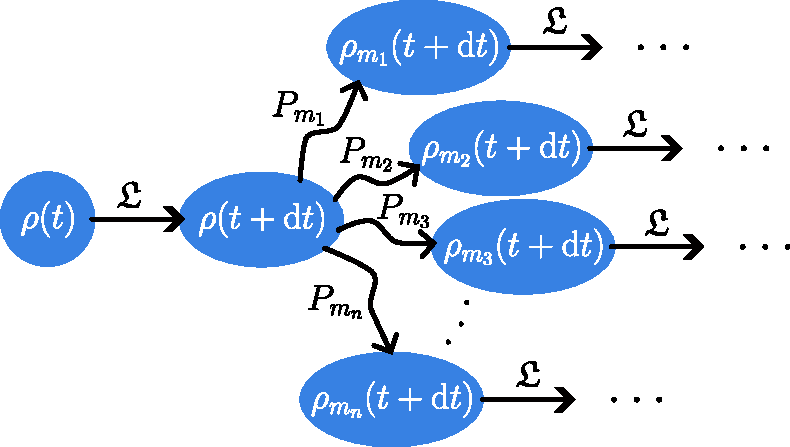
\includegraphics[width=0.7\textwidth]{Images/QT.pdf}
	\begin{example}
	The outcome of the measurement is labelled by $m$ and there are $n$ possible outcomes. 
	\end{example}
	\begin{alertblock}{A single trajectory}
		We follow one trajectory among all the possible trajectories!
	\end{alertblock}
\end{frame}

\subsection{Photo-detection}
\begin{frame}
	\frametitle{Unravelling the photo-detection Stochastic Master Equation (SME)}
	By projecting the environment onto the basis $\qty{\ket{m}}_{m\in\mathbb{N}}$ at each time step, the possible measurement outcomes are $\mathrm{d}N_t=0$ or $\mathrm{d}N_t=1$.
	\begin{block}{$\mathrm{d}N_t$ is a Poisson increment (follows a Poisson distribution)}
		\begin{equation*}
			\mathrm{d}N_t^2=\mathrm{d}N_t,\quad \mathbb{V}\qty[\mathrm{d}N_t]\approx\mathbb{E}\qty[\mathrm{d}N_t]=\textcolor{red}{\expval{c^\dagger c}_t} k \mathrm{d}t.
		\end{equation*}
	\end{block}
	We define for all operator $c$ and for all density matrix $\rho$, $\mathfrak{H}[c]\rho = c\rho+\rho c^\dagger - \expval{c+c^\dagger}_t \rho$.
	\begin{alertblock}{Photo-detection SME}
		\begin{equation*}
			\mathrm{d}\rho_c = -i\qty[H_S, \rho]\mathrm{d}t-\frac{k}{2}\mathfrak{H}\qty[c^\dagger c]\rho_c\mathrm{d}t + \qty(\frac{c\rho_c c^\dagger}{\expval{c^\dagger c}_t}-\rho_c)\mathrm{d}N_t.
		\end{equation*}
	\end{alertblock}
\end{frame}

\subsection{Homodyne detection}
\begin{frame}
	\frametitle{Unravelling the homodyne detection SME}
	By projecting the environment onto the continuous basis $\qty{\ket{x_\theta}_t}_{x_\theta\in\mathbb{R}}$ at each timestep, the possible measurement outcomes span the entire real axis.
	\begin{block}{The quadrature operator $\hat{x}_\theta$ and the measurement signal $\mathrm{d}y_t$}
		\begin{equation*}
			\hat{x}_\theta = \frac{B_t e^{-i\theta}+B_t^\dagger e^{i\theta}}{\sqrt{2}}\quad\Longrightarrow\quad\mathrm{d}y_t = \sqrt{k}\textcolor{red}{\expval{ce^{-i\theta}+c^\dagger e^{i\theta}}_t}\mathrm{d}t+\mathrm{d}w_t.
		\end{equation*}
	\end{block}
	\begin{block}{$\mathrm{d}w_t$ is a Wiener increment (follows a Gaussian distribution)}
		\begin{equation*}
			\mathrm{d}w_t^2=\mathrm{d}t,\quad \mathbb{V}\qty[\mathrm{d}w_t]=\mathrm{d}t,\quad \mathbb{E}\qty[\mathrm{d}w_t]=0.
		\end{equation*}
	\end{block}
	\begin{alertblock}{Homodyne detection SME}
		\begin{equation*}
			\mathrm{d}\rho_c = -i\qty[H_S, \rho]\mathrm{d}t-\frac{k}{2}\mathfrak{D}\qty[c]\rho_c\mathrm{d}t + \sqrt{k}\mathfrak{H}\qty[ce^{-i\theta}]\rho_c \mathrm{d}w_t.
		\end{equation*}
	\end{alertblock}
\end{frame}
\subsection{Kraus operators}
\begin{frame}
	\frametitle{The Kraus operators formalism}
	By using a different formalism representing the effects of measurement, we can rewrite non-normalized state evolutions.
	\begin{block}{Photo-detection conditional evolutions}
		\begin{align*}
			\ket{\tilde{\psi}_0(t+\mathrm{d}t)}&=K_0 \ket{\tilde{\psi}_c(t)}=\qty[\mathbb{I}-\qty(\frac{k}{2}c^\dagger c+iH_S)\mathrm{d}t]\ket{\tilde{\psi}_c(t)},\\
			\ket{\tilde{\psi}_1(t+\mathrm{d}t)}&=K_1 \ket{\tilde{\psi}_c(t)}=\sqrt{k\mathrm{d}t}c\ket{\tilde{\psi}_c(t)}.
		\end{align*}
	\end{block}
	$\Longrightarrow$ the Monte Carlo method.
	\begin{block}{Homodyne detection conditional evolution}
		\begin{equation*}
			\tilde{\rho}_c(t+\mathrm{d}t) = K_{dy_t}\rho_c(t)K_{dy_t}^\dagger,
		\end{equation*}
		where $K_{dy_t} = \mathbb{I}-iH_S\mathrm{d}t-\frac{k}{2}c^\dagger c\mathrm{d}t + \sqrt{k}c\mathrm{d}y_t$.
	\end{block}
\end{frame}

\section{Simulations}
\begin{frame}{The qubit under photo-detection of its environment}
	\centering
	$\ket{\psi(0)}=\frac{\ket{e}+\ket{g}}{\sqrt{2}}$
	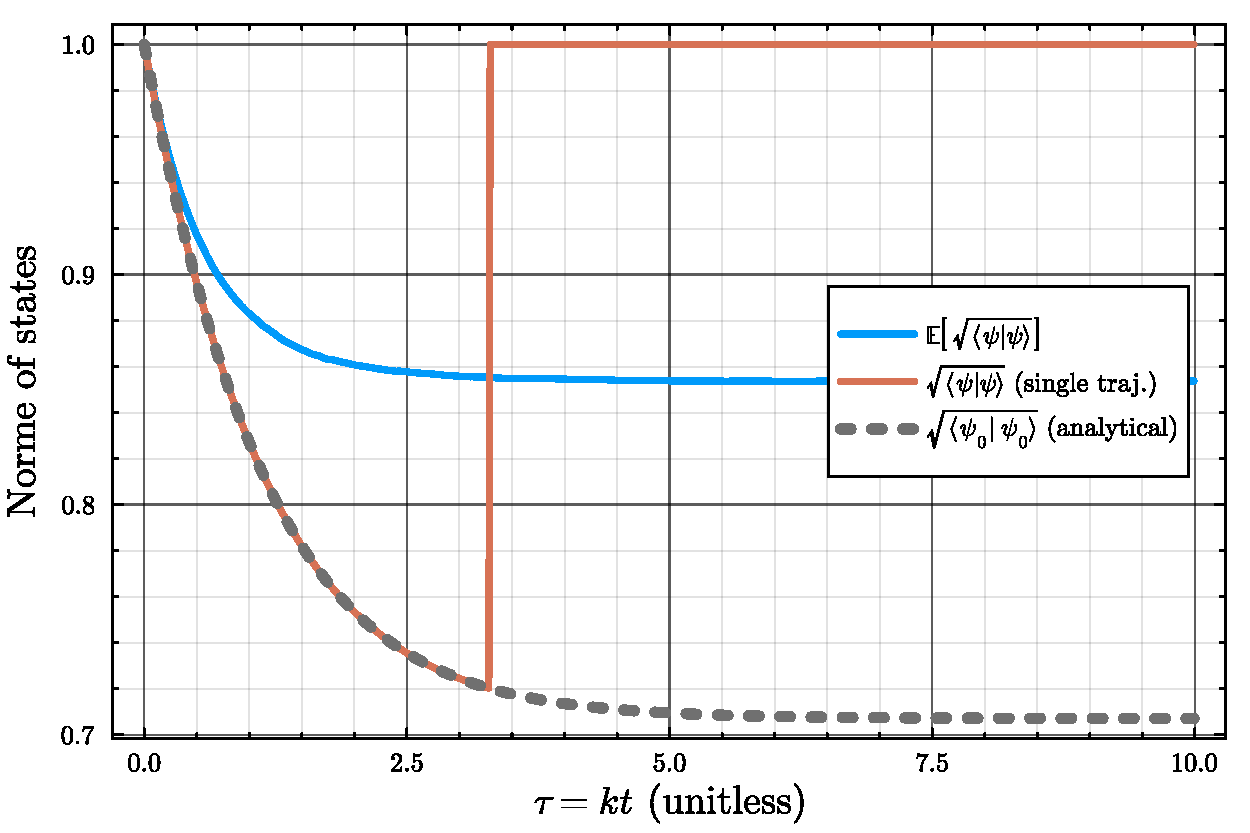
\includegraphics[width=\linewidth]{MCQ/NormeSuperposition.pdf}
\end{frame}
% \begin{frame}{The qubit under photo-detection of its environment}
% 	\centering
% 		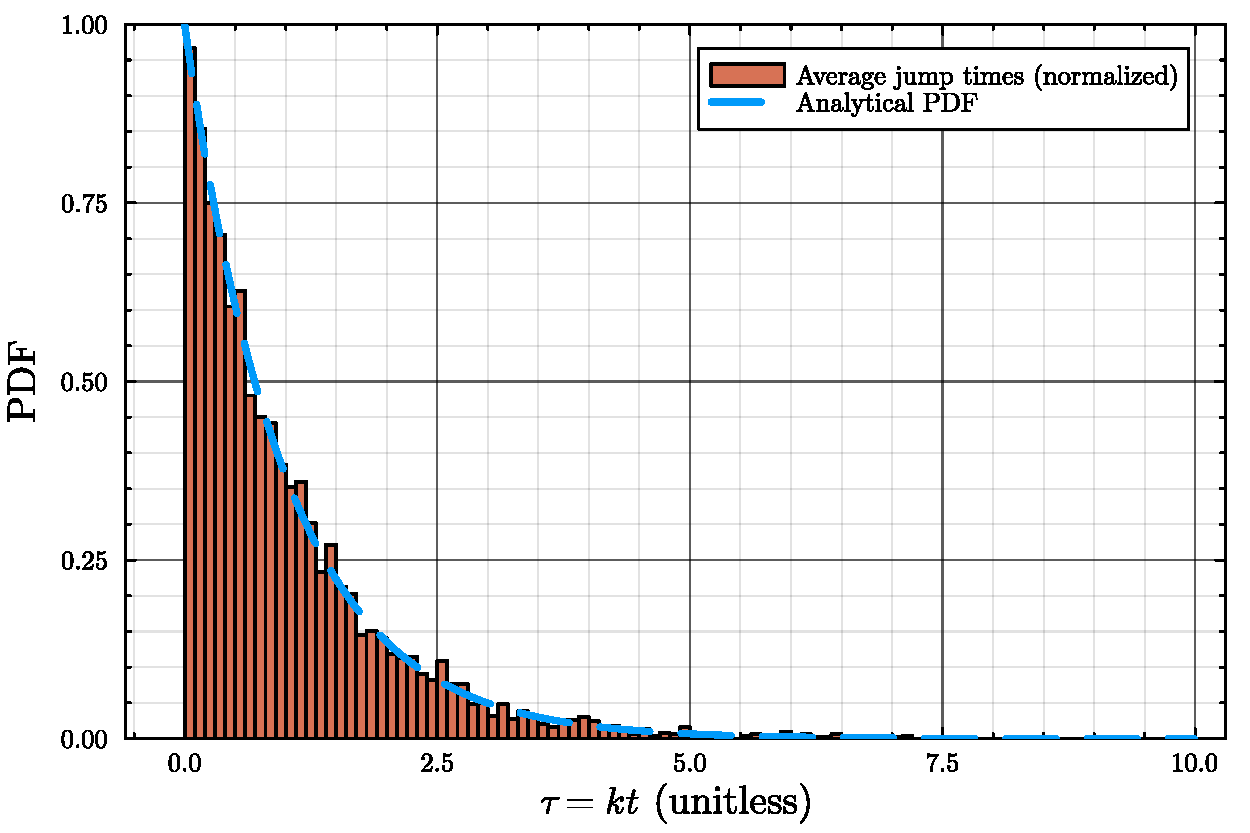
\includegraphics[width=\linewidth]{MCQ/histo.pdf}
% \end{frame}
\begin{frame}{The qubit under photo-detection of its environment}
	\centering
		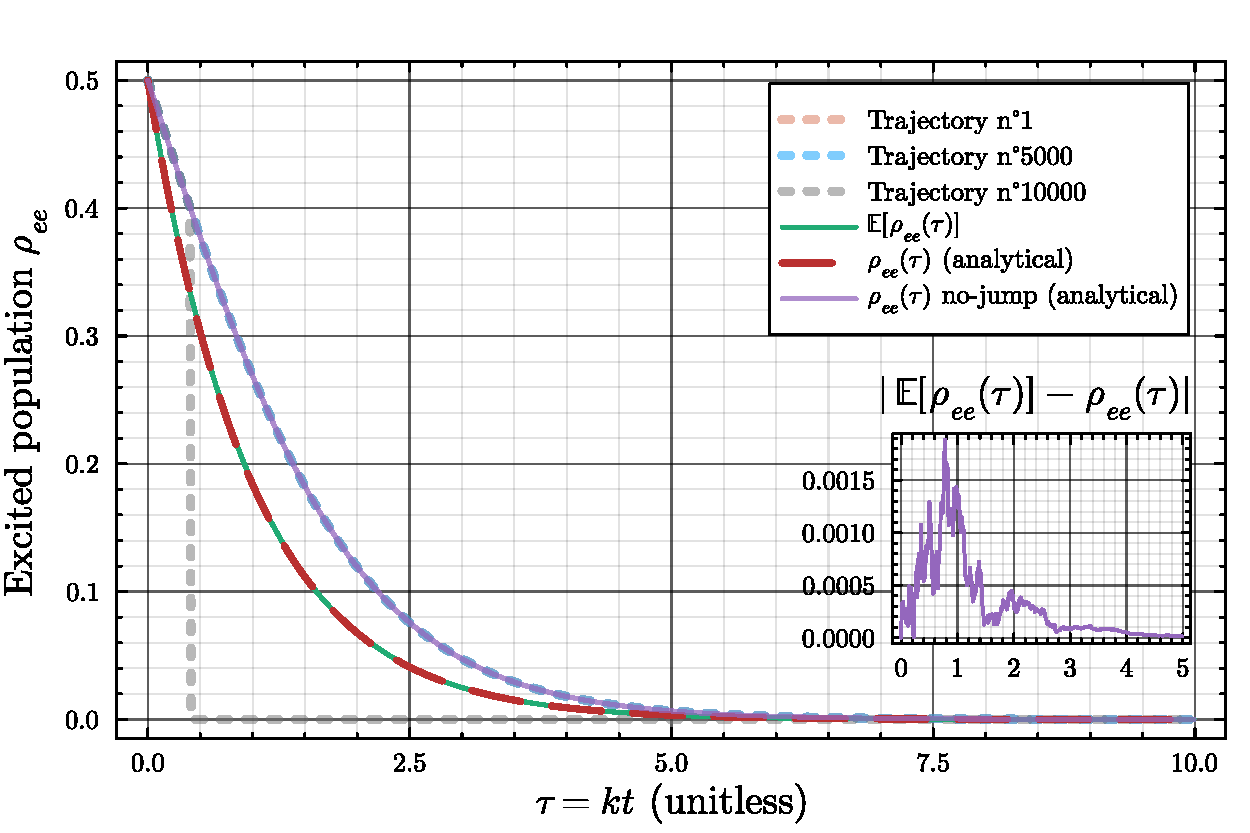
\includegraphics[width=\linewidth]{MCQ/Pop_10000.pdf}
\end{frame}

\begin{frame}{The qubit under homodyne detection of its environment}
	\centering
	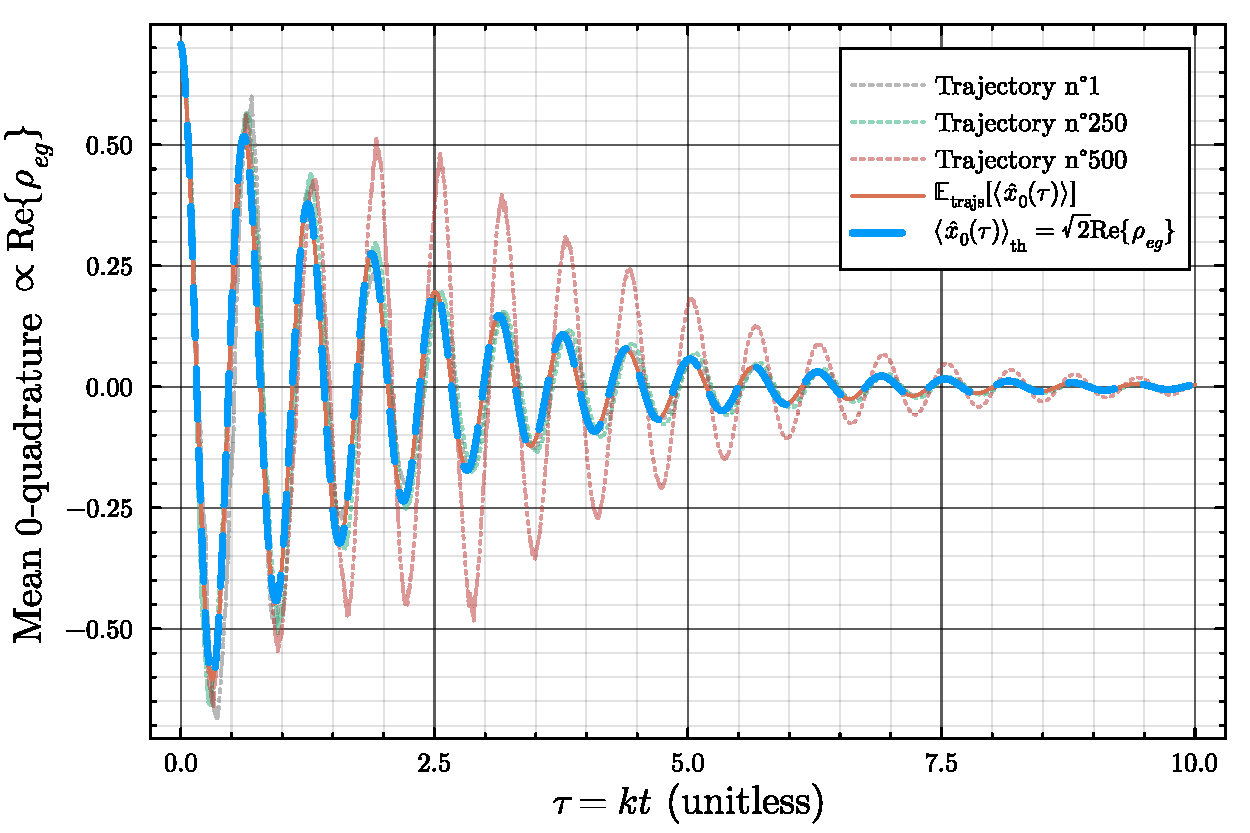
\includegraphics[width=\linewidth]{HQ/Xquadrature.pdf}
\end{frame}
\begin{frame}{The qubit under homodyne detection of its environment}
	\centering
	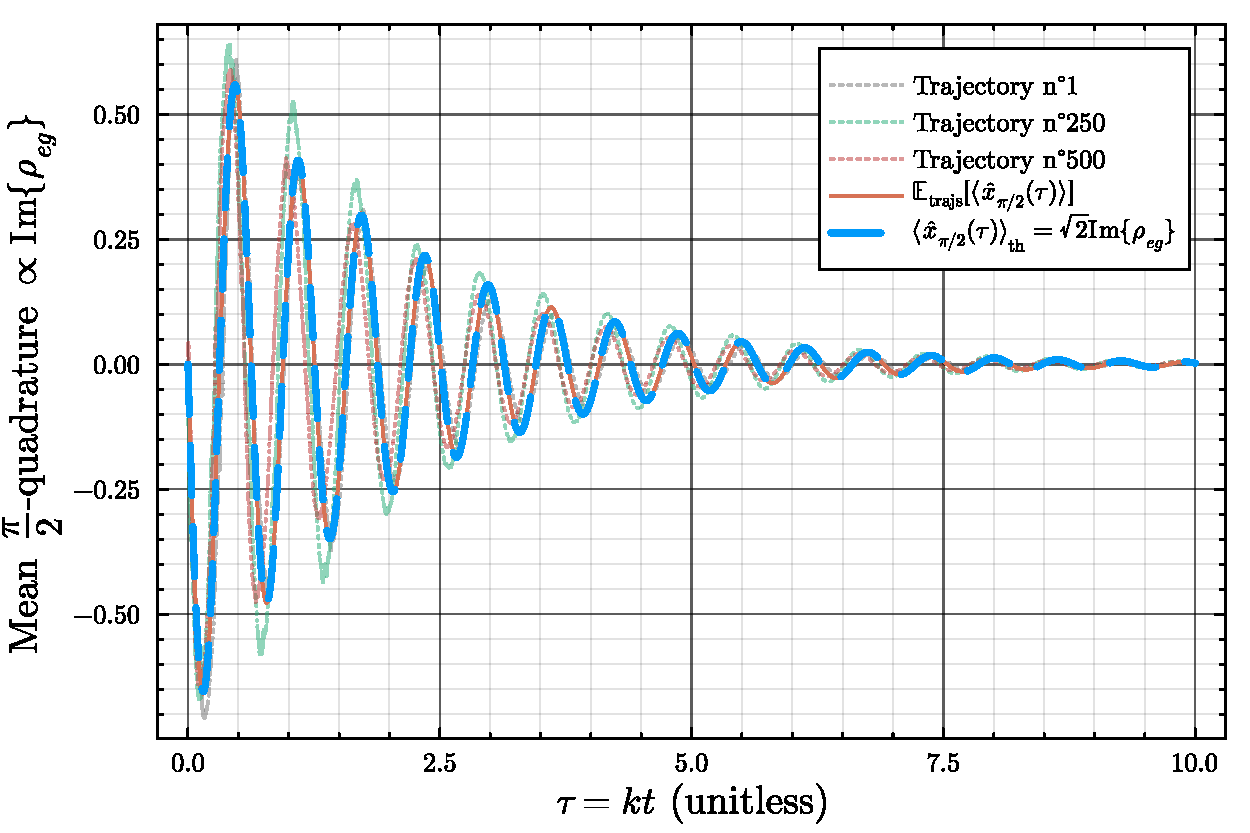
\includegraphics[width=\linewidth]{HQ/Pquadrature.pdf}
\end{frame}



\section{Conclusion}
\begin{frame}{Conclusion}
	\begin{itemize}[label=$\blacktriangleright$]
		\item Stochastic master equations and conditional trajectories.
		\item Unravellings of the unconditional master equation.
		\item Obtaining pieces of information about the system in average via weak measurements.
	\end{itemize}\pause\vfill
	\begin{itemize}[label=$\bullet$]
		\item We used very ideal approximations.
		\item What about inefficient detectors?
		\item Is there any other measuring process?
		\item What about thermal noises?
	\end{itemize}\pause
	\vfill\centering\Large
	Thank you for your time and attention.
\end{frame}

\appendix\backupbegin\setbeamercolor{page number in head/foot}{fg=white}
\section*{Appendices}
\begin{frame}
	\vfill
	\centering\Huge
	Appendices
	\vfill
\end{frame}
\subsection{The harmonic oscillator}
\begin{frame}{The harmonic oscillator under photo-detection of its environment}
	\centering
		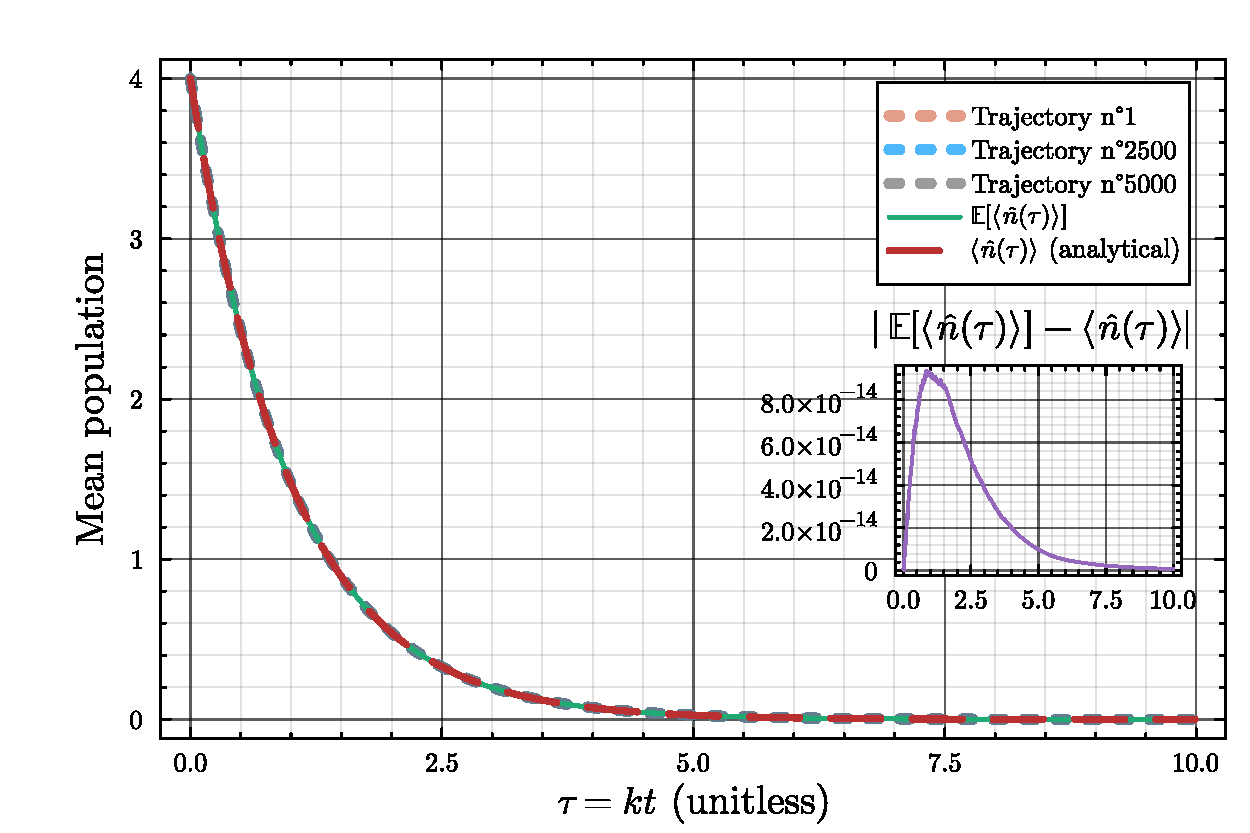
\includegraphics[width=\linewidth]{MCH/Pop_5000.pdf}
\end{frame}
\begin{frame}{The harmonic oscillator under photo-detection of its environment}
	\centering
		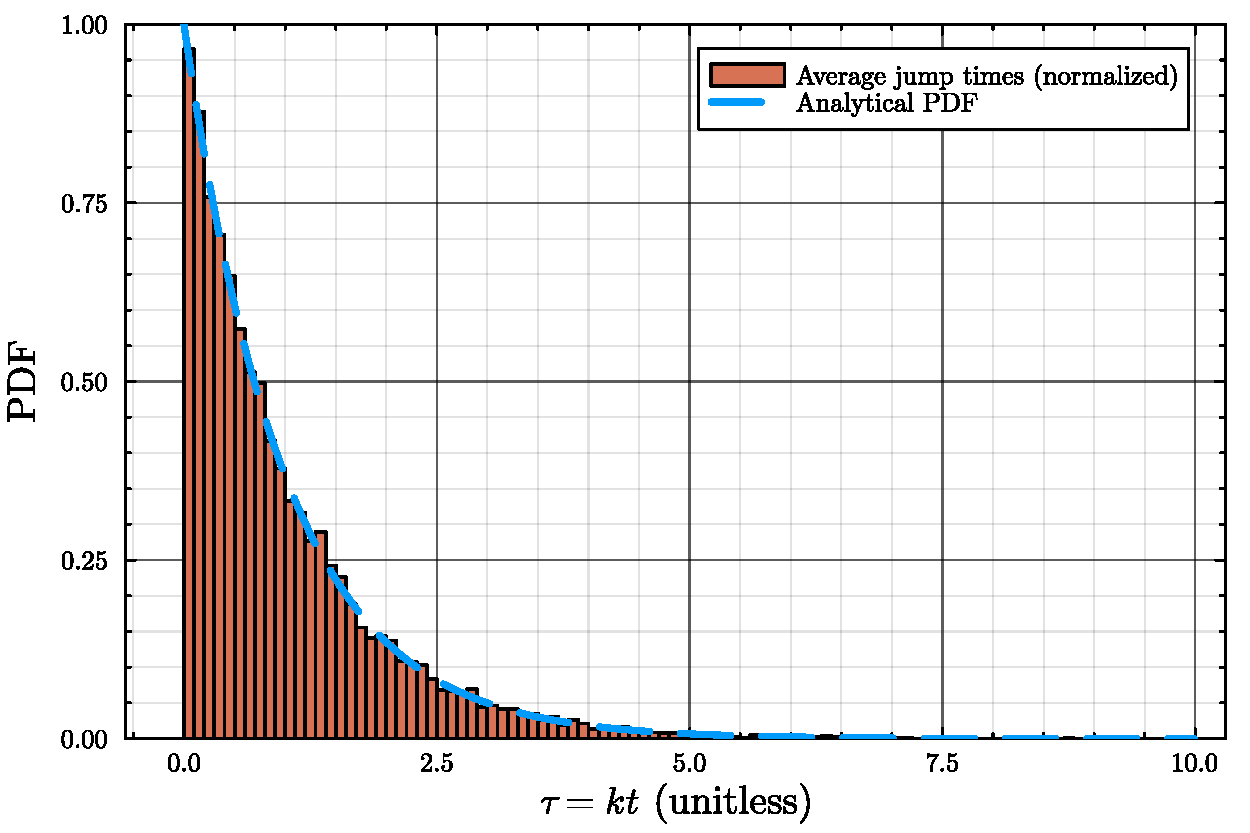
\includegraphics[width=\linewidth]{MCH/histo.pdf}
\end{frame}
\begin{frame}{The harmonic oscillator under homodyne detection of its environment}
	\centering
	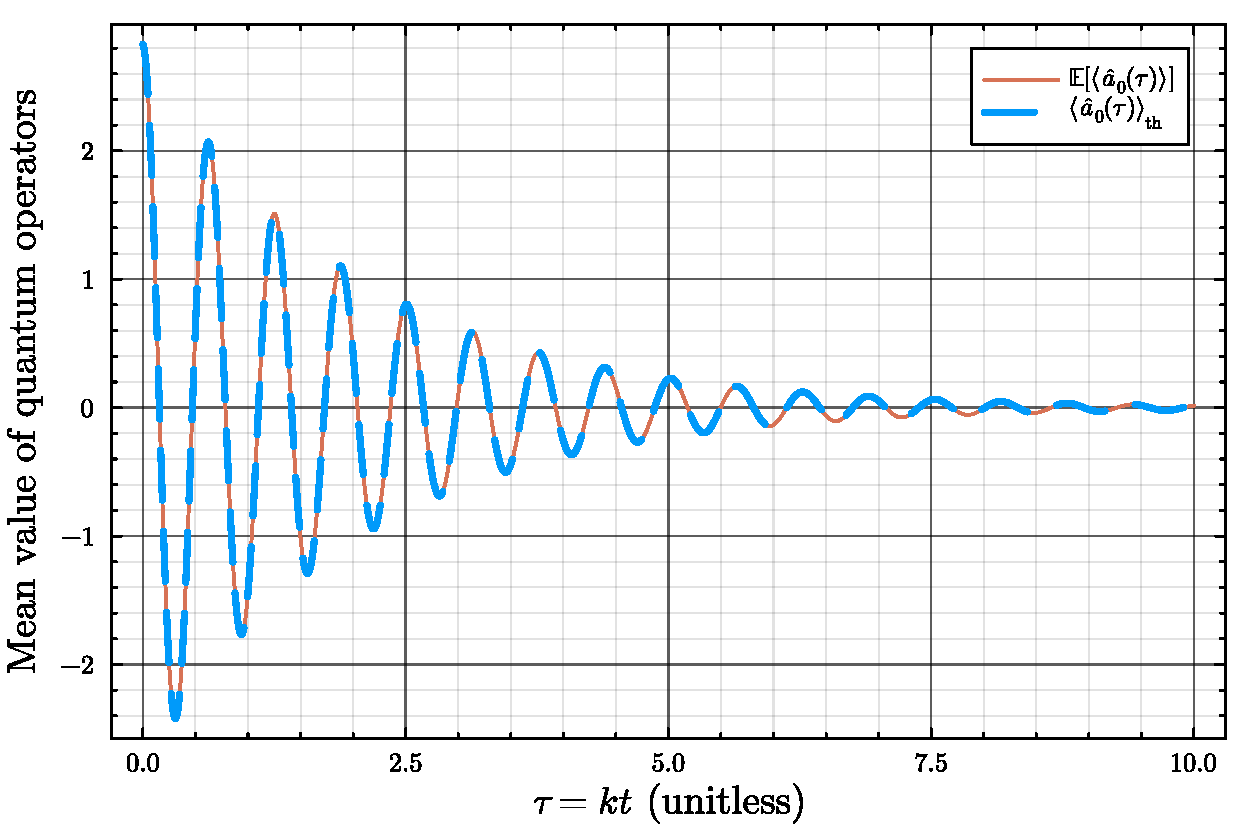
\includegraphics[width=\linewidth]{HH/Xquadrature.pdf}
\end{frame}
\begin{frame}{The harmonic oscillator under homodyne detection of its environment}
	\centering
	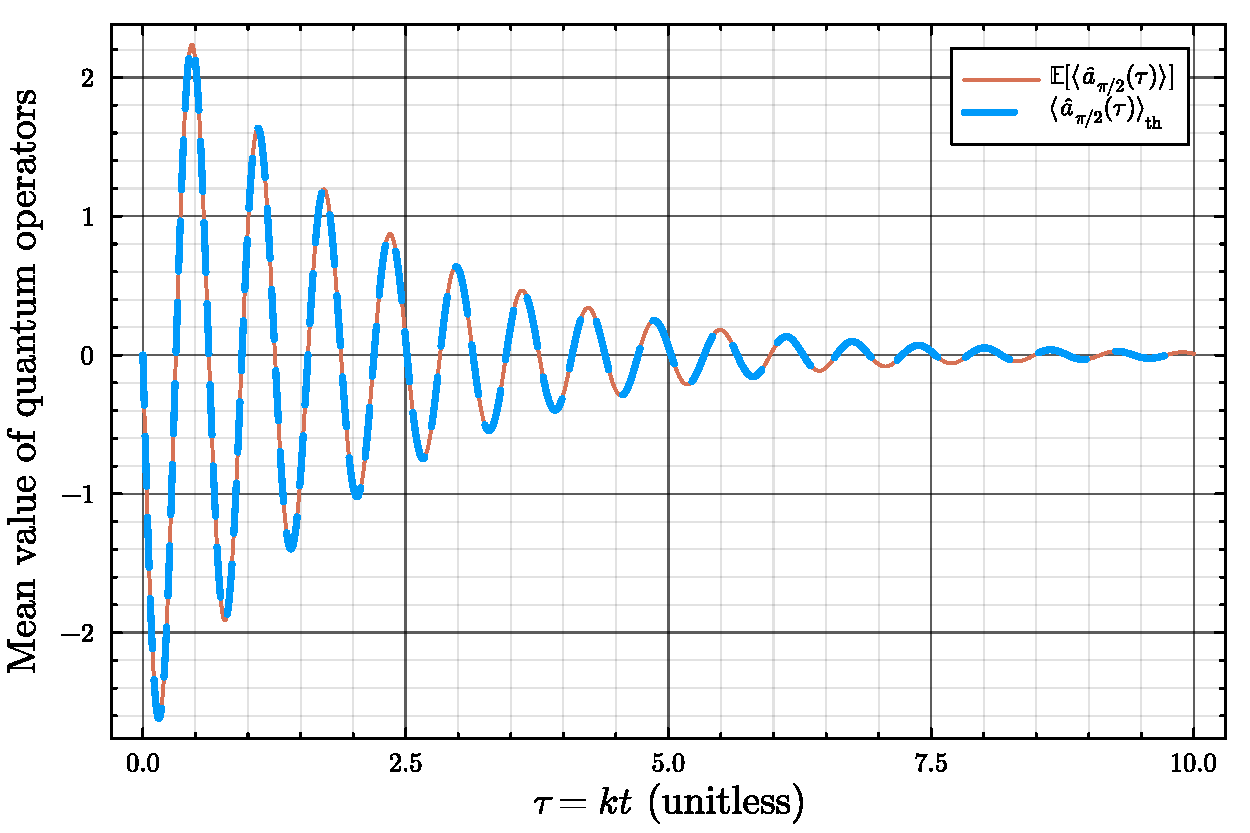
\includegraphics[width=\linewidth]{HH/Pquadrature.pdf}
\end{frame}
\begin{frame}{The harmonic oscillator under homodyne detection of its environment}
	\centering
	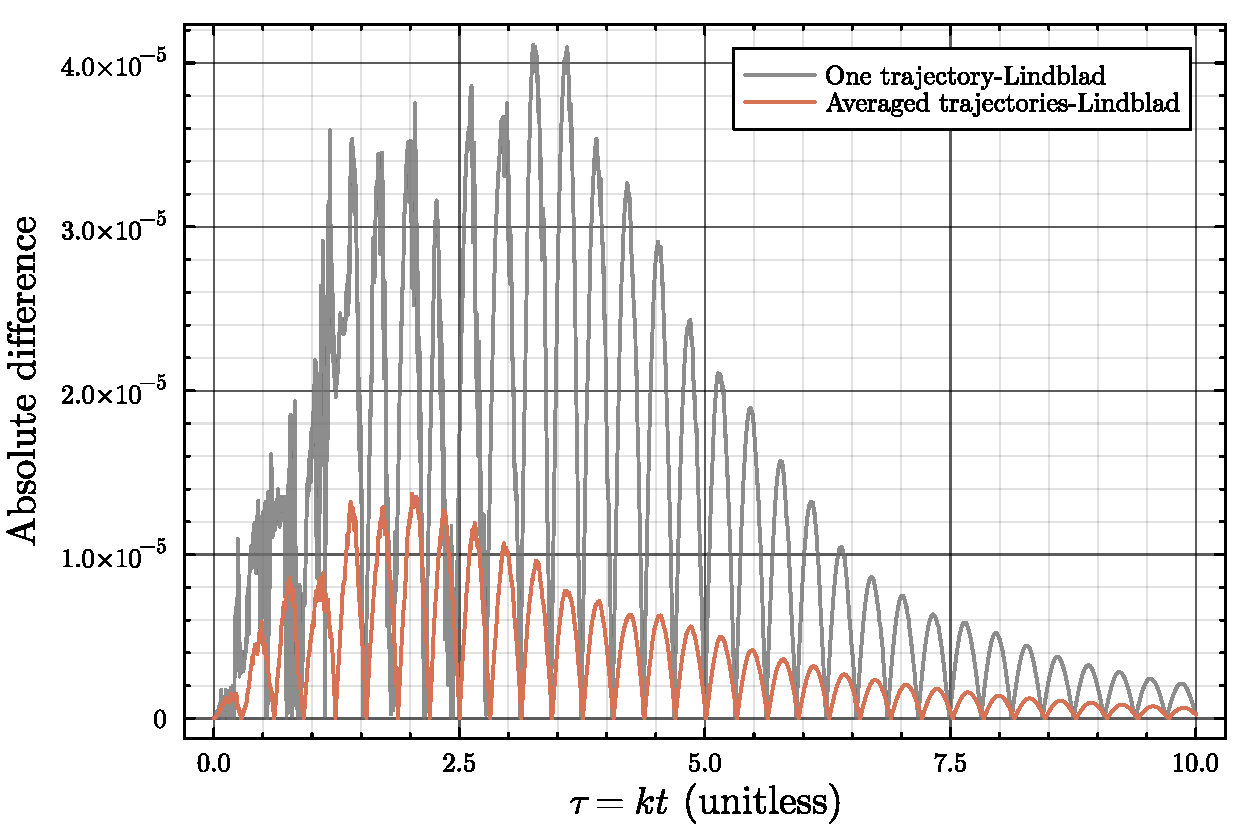
\includegraphics[width=\linewidth]{HH/XquadSingleError.pdf}
\end{frame}
\begin{frame}{The harmonic oscillator under homodyne detection of its environment}
	\centering
	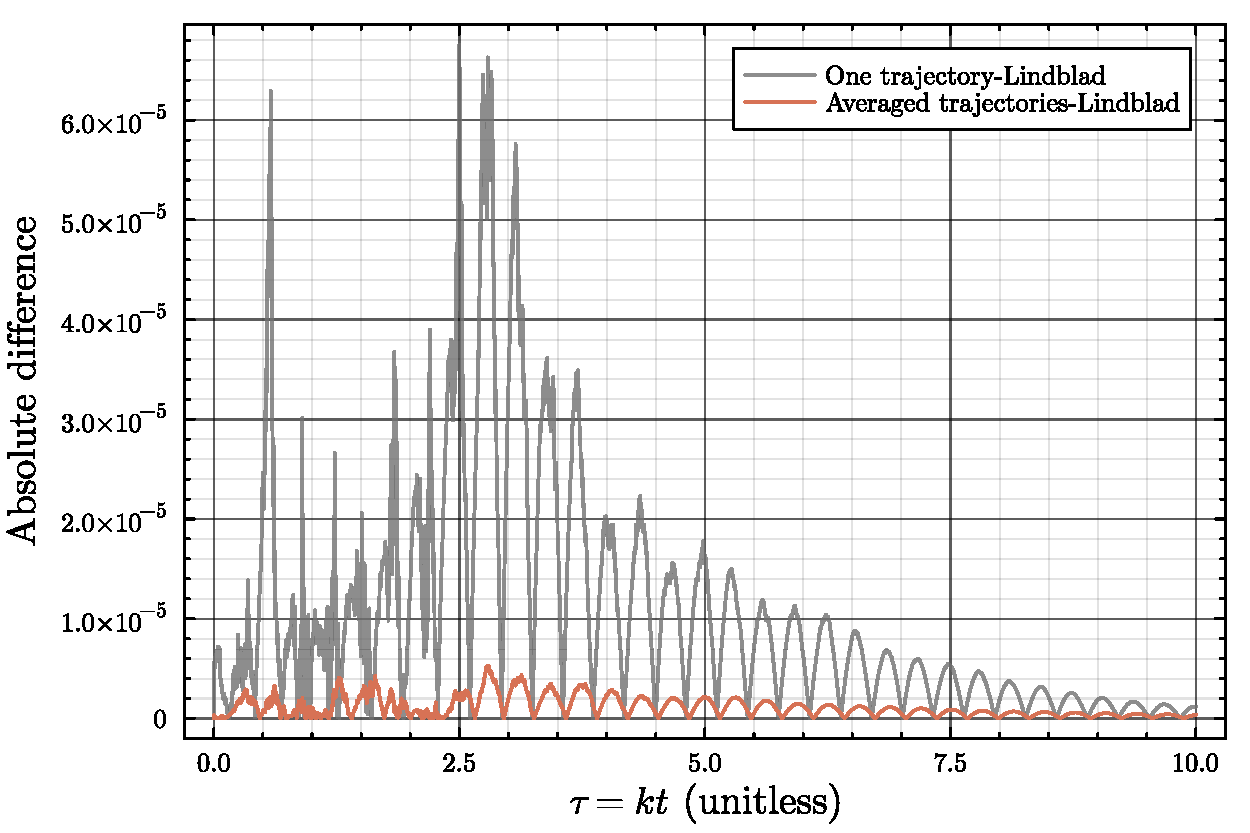
\includegraphics[width=\linewidth]{HH/PquadSingleError.pdf}
\end{frame}
\begin{frame}{The qubit under homodyne detection of its environment}
	\centering
	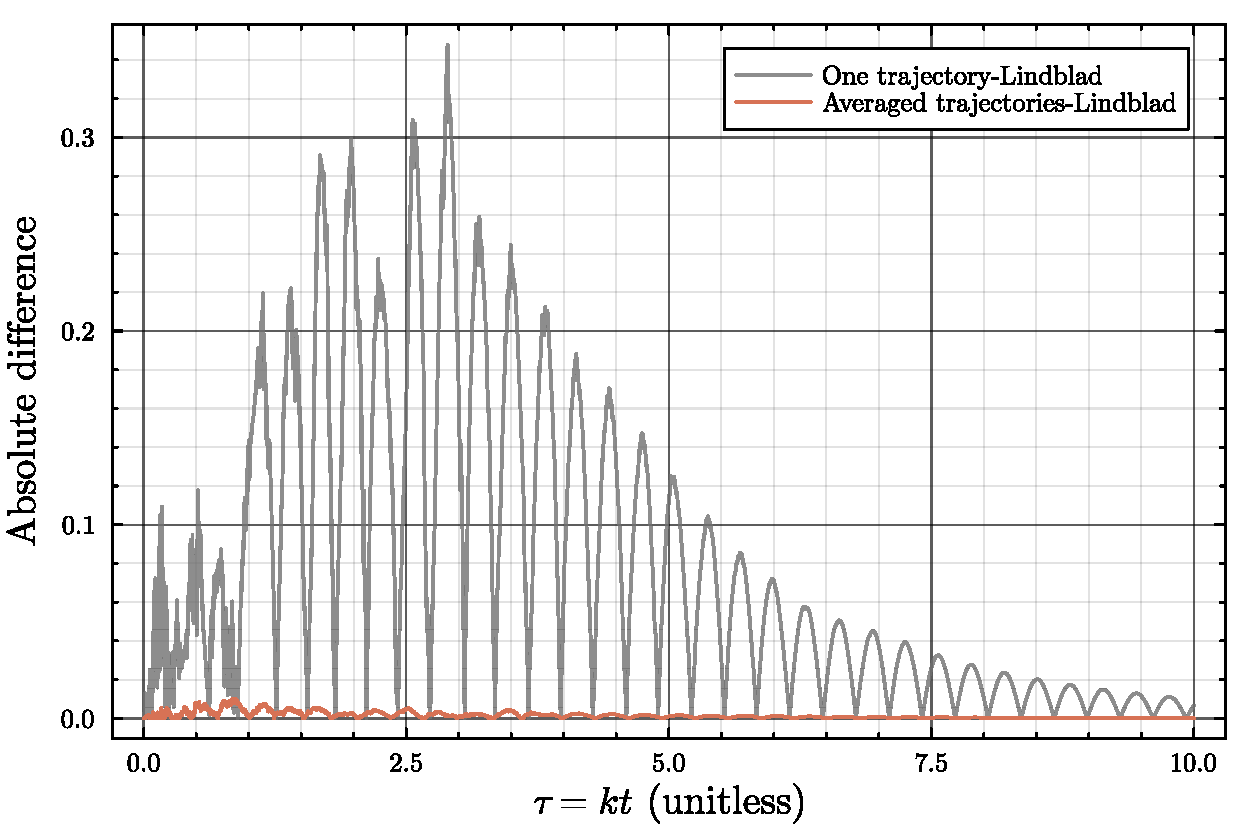
\includegraphics[width=\linewidth]{HQ/XquadSingleError.pdf}
\end{frame}
\begin{frame}{The qubit under homodyne detection of its environment}
	\centering
	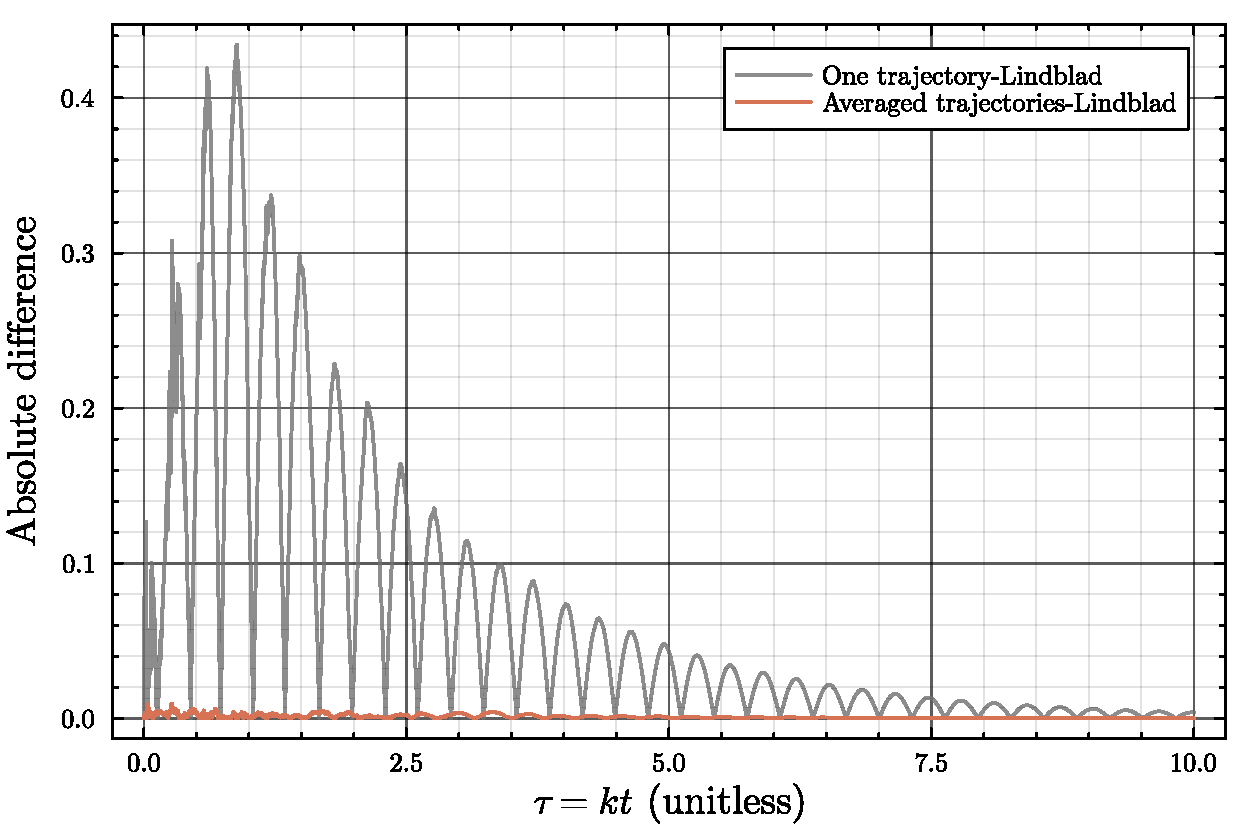
\includegraphics[width=\linewidth]{HQ/PquadSingleError.pdf}
\end{frame}
\begin{frame}
	\frametitle{Linearization of the SMEs}
	We can find the linear equations describing the evolution of states according to the photo-detection/homodyne detection. However this is possible \textbf{at the cost of the normalization of the state}.
	\begin{block}{Linear photo-detection SME}
		\begin{equation*}
			\mathrm{d}\breve{\rho}_c = -i\qty[H_S, \breve{\rho}_c]\mathrm{d}t - \frac{k}{2}\qty{c^\dagger c, \breve{\rho}_c}\mathrm{d}t + k\breve{\rho}_c\mathrm{d}t + \qty(c\breve{\rho}_c c^\dagger - \breve{\rho}_c)\mathrm{d}N_t.
		\end{equation*}
	\end{block}
	\begin{block}{Linear homodyne detection SME}
		\begin{equation*}
			\mathrm{d}\breve{\rho}_c = -i\qty[H_S, \breve{\rho}_c]\mathrm{d}t +k \mathfrak{D}[c]\breve{\rho}_c(t) + \sqrt{k}\qty(ce^{-i\theta}\breve{\rho}_c+\breve{\rho}_c c^\dagger e^{i\theta})\mathrm{d}w_t.
		\end{equation*}
	\end{block}
Every statistical quantity follows \textit{ostensible} probability law instead of the \textit{true} probability law in the linear (non-normalized) case.
\end{frame}
\begin{frame}{The qubit under photo-detection of its environment}
	\centering
	$\ket{\psi(0)}=\ket{e}$
	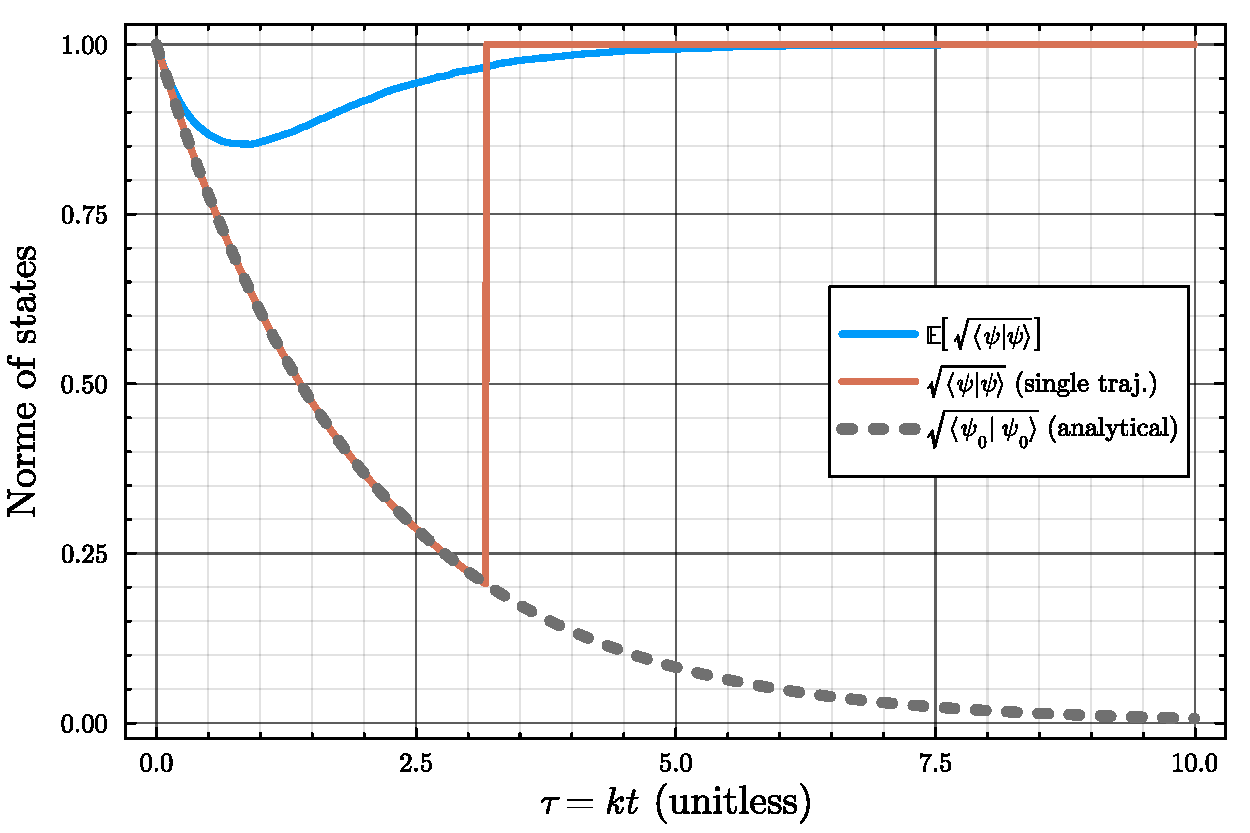
\includegraphics[width=\linewidth]{MCQ/NormeE.pdf}
\end{frame}
\begin{frame}{The homodyne measurement setup}
	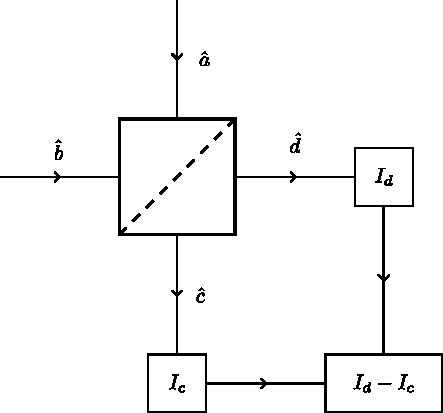
\includegraphics[width=0.8\textwidth]{Images/Homodyne.pdf}
\end{frame}
\section*{Bibliography}
\begin{frame}{Bibliography}
	\printbibliography
\end{frame}
\backupend
\end{document}

